\begin{frame}{Fonds Charcot}
\begin{block}{SorbonNum\footnote{\tiny{\url{https://patrimoine.sorbonne-universite.fr/}}} -- Bibliothèque de Sorbonne Université (BSU)}
201 documents XML OCRisés (sans post-correction)
\end{block}
\begin{itemize}
    \item \og{}Charcot\fg{} : textes rédigés par Charcot
    \item \og{}Autres\fg{} : textes rédigés par son réseau scientifique
\end{itemize}
\begin{table}[!ht]
    \centering
    \begin{tabular}{|c|c|c|}
    \hline 
    \rowcolor{gray!30}
       Corpus & Nb de docs & Nb de tokens \\
       \hline
       \og{}Charcot\fg{}  & 68 & 12 190 649 (38,12\%) \\
       \og{}Autres\fg{}  & 133 & 19 788 830 (61,88\%) \\
       \hline\hline
       \textbf{Total} & \textbf{201} & \textbf{31 979 479} (100\%)\\
       \hline
    \end{tabular}
    \caption{Répartition du corpus issu du fonds Charcot\footnote{\tiny{\url{https://patrimoine.sorbonne-universite.fr/collection/Fonds-Charcot}}}.}
    \label{tab:my_label}
\end{table}
\end{frame}


\begin{frame}{Mesurer le degré d'intertextualité}
Mesurer informatiquement l'impact de Charcot sur son réseau $\rightarrow$ intertextualité uni-directionnelle
\begin{figure}[!h]
    \centering
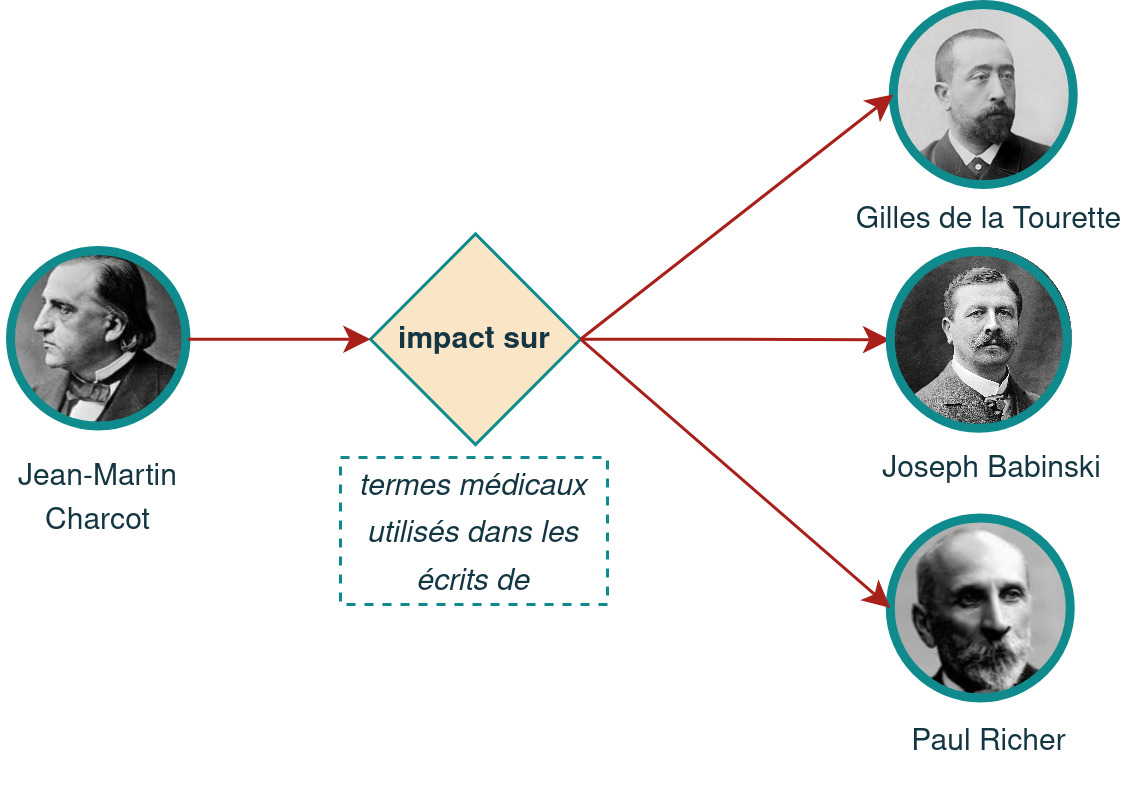
\includegraphics[width=80mm,scale=0.5]{pic/charcot_intertextualite.jpg}
    \caption{Opérationnalisation de l'impact de Charcot sur ses élèves.}
    \label{fig:my_label}
\end{figure}
\end{frame}

\begin{frame}{Première analyse}
\textbf{OBVIE}\footnote{\url{https://obtic.huma-num.fr/obvie/}}
\begin{itemize}
    \item moteur de recherche permettant la fouille avancée des corpus en \textsc{XML-TEI}
    \item identification des substantifs les plus importants de chaque corpus 
    \begin{itemize}
        \item fréquences brutes, mesures \textsc{TF-IDF}, \textsc{BM25}, $\chi^2$, Test Gamma
    \end{itemize}
    \item repérage des textes similaires par ordre de pertinence à partir des termes en commun
\end{itemize}
    
\end{frame}
\begin{frame}{OBVIE -- Corpus Charcot\footnote{\url{https://obtic.huma-num.fr/obvie/charcot/?view=corpus}}}
\danger impossible de quantifier l'importance des MWEs
\begin{figure}[!h]
    \centering
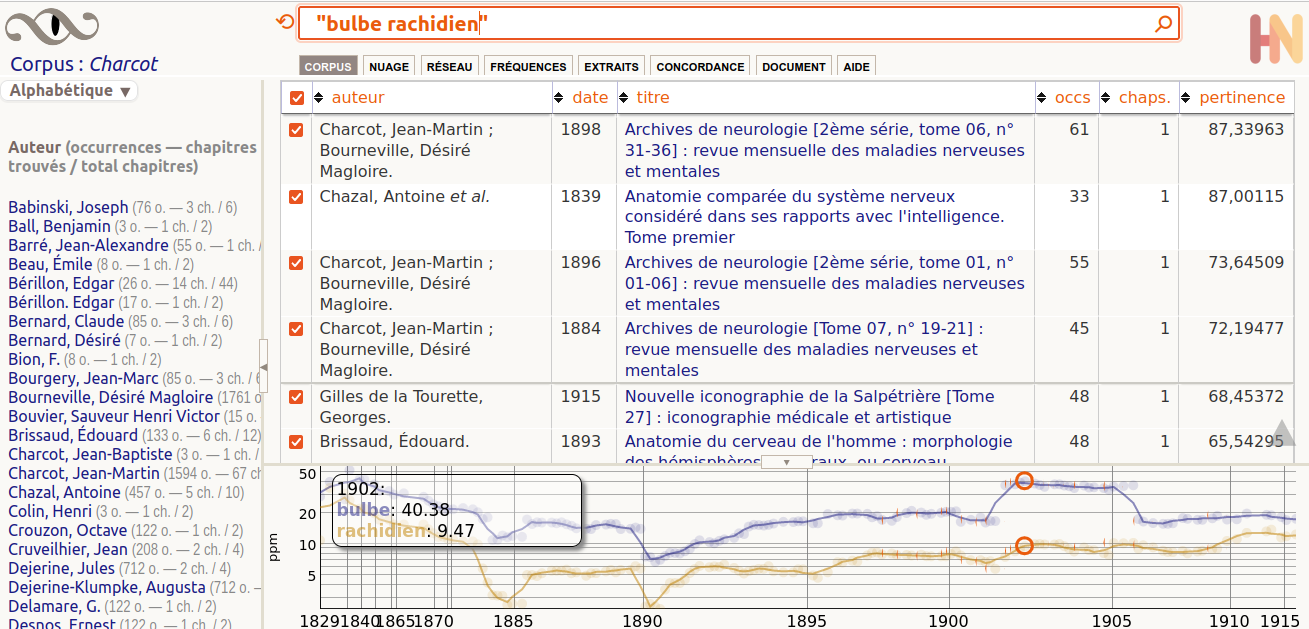
\includegraphics[width=90mm,scale=0.5]{pic/bulbe_rachidien.png}
    \caption{Distribution des fréquences des tokens avec la frise chronologique pour ceux constituant l'expression \textit{bulbe rachidien} (issus des corpus \og{}Charcot\fg{} et \og{}Autres\fg{}).}
    \label{fig:my_label}
\end{figure}
% citations directes (\cite{manjavacas2019})
\end{frame}

\begin{frame}{Deuxième analyse}
    \textbf{TextPair}\footnote{\url{https://artfl-project.uchicago.edu/text-pair}}
    \begin{itemize}
        \item alignement des séquences similaires dans les deux corpus
        \item génère une liste de passages similaires pour chaque texte
        \item séquences de mots qui se chevauchent (trigrammes de mots)
        \item comparer ces résultats avec ceux de séquences dans d’autres textes
    \end{itemize}
\end{frame}

\begin{frame}{Deuxième analyse -- TextPair\footnote{\url{https://anomander.uchicago.edu/text-pair/charcot2autres/}}}
\danger nombre de
résultats assez conséquent -- filtrage nécessaire
    \begin{figure}[!ht]
        \centering
        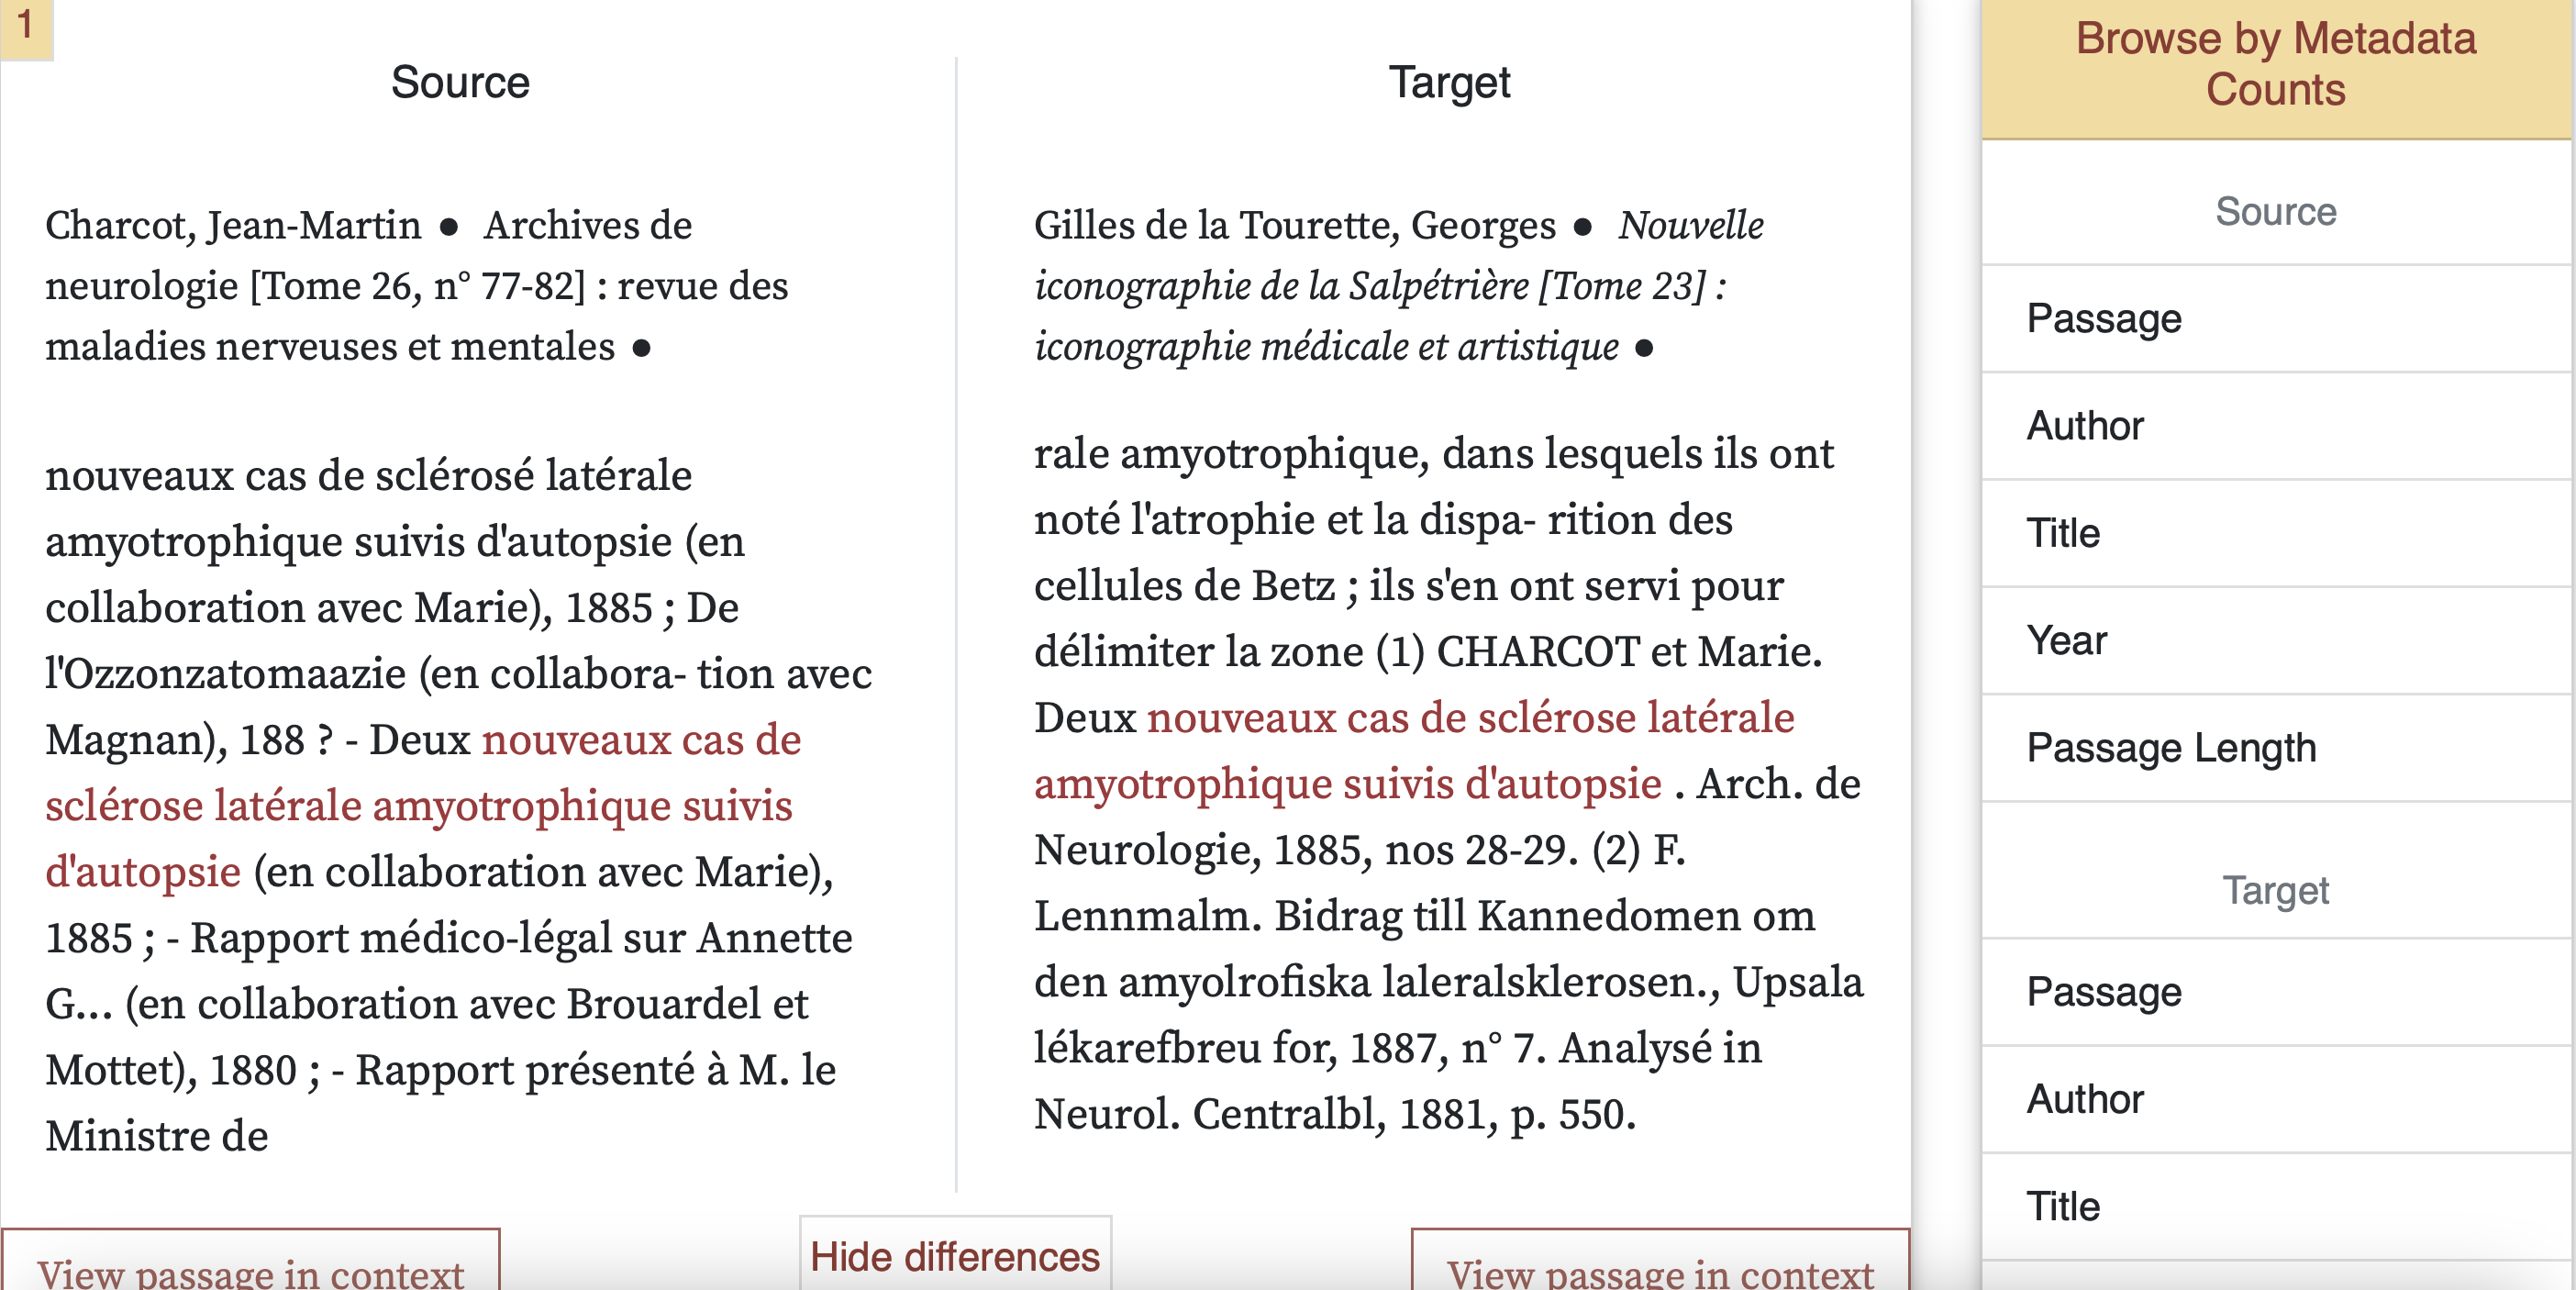
\includegraphics[width=90mm,scale=0.5]{pic/textpair.png}
        \caption{Alignement et comparaison des textes de
Charcot à celui de Georges Gilles de la Tourette (le seul
résultat) en lançant la requête \textit{sclérose latérale
amyotrophique}.}
        \label{fig:enter-label}
    \end{figure}
\end{frame}
